\documentclass[12pt,numbers=noenddot,parskip,bibliography=totocnumbered,listof=totocnumbered]{scrreprt}
\usepackage[paper=a4paper,left=30mm,right=25mm,top=30mm,bottom=30mm]{geometry}
\usepackage[utf8]{inputenc}
\usepackage[hyphens]{url}
\usepackage[english]{babel}
\DeclareTOCStyleEntry[entrynumberformat=\adddot]{tocline}{figure}
\newcommand*{\adddot}[1]{#1\unskip.\hfil}
\usepackage{lmodern}
\usepackage[sort&compress]{natbib}
\usepackage{graphicx} 
\usepackage{subcaption}
\usepackage{rotating}
\usepackage{pgfplots}
\pgfplotsset{compat=newest}
\usepackage{transparent}
\usepackage{multirow}
\usepackage{scrextend}
\usepackage{tabularx}
\usepackage{pifont}
\usepackage{enumitem}
\usepackage{setspace}
\usepackage{amsmath}
\usepackage[automark]{scrlayer-scrpage}
\pgfplotstableset{col sep=semicolon}

% Stil der Seiten
\pagestyle{scrheadings}
\clearscrheadfoot

%Abstand der Fussnoten
\deffootnote{1em}{1em}{\textsuperscript{\thefootnotemark\ }}

%Zeilenabstand
\onehalfspacing

%Regeln, bis zu welcher Tiefe Überschriften angezeigt werden sollen (Anzeige der Überschriften im Verzeichnis / Anzeige der Nummerierung)
\setcounter{tocdepth}{3}
\setcounter{secnumdepth}{3}

%Kopfzeile (Kapitel / Standard)
\ohead{\transparent{0.5}\headmark\transparent{0.5}\transparent{1}}

%Fußzeile (Kapitel / Standard)
\ofoot[\rlap{\hspace{.5cm}\rule[-0.7ex]{.8pt}{\baselineskip}\hspace{.5cm}\pagemark}]{\rlap{\hspace{.5cm}\rule[-0.7ex]{.8pt}{\baselineskip}\hspace{.5cm}\pagemark}}

%Kapitel in Kopfzeile ohne Zahl
\renewcommand*{\chaptermarkformat}{}

%Schriftarten
\addtokomafont{pagenumber}{\sffamily \upshape}
\addtokomafont{pageheadfoot}{\sffamily \upshape}\usepackage[defaultfam,light,tabular,lining]{montserrat}
\usepackage[T1]{fontenc}
\renewcommand*\oldstylenums[1]{{\fontfamily{Montserrat-TOsF}\selectfont #1}}

% Auflistungen
\setkomafont{labelinglabel}{\textit}

\begin{document}
	
% TItelseite
\begin{titlepage}
\null
\vfill
% The Collective Guide: A machine for collective recommendations and its desire for disclosure
% Honestly transforms experiences in a collective into public recommendations
% The Honest Machine: Transforms experiences in a collective into honest recommendations
% The bold attempt of transforming experiences in a collective into  recommendations
% The Honest Machine: The attempt of converting experiences in a collective into honest recommendations

% Felix: Sollte beinhalten...
% Recommendation
% Virtuell vernetzt bzw. wohnt im Netz
% Keine Negation
% Freizeitgestaltung verbessern

\Huge\textsf{\textbf{Free your free time
\vspace{0.5em}}}\\
\LARGE\textsf{ Assessment of a recommendation machine to increase 
%one's quota of 
the amount of
spare time spent collectively 
%and in person 
} \vspace{1.5em}\\
\Large\textsf{Jan-Hendrik Wolf}
\vfill
\vfill
\vfill
\small{Thesis submitted to the University Bremen in partial fulfillment of the requirements for a M.Sc. degree in Digital Media\\
Bremen, 30. Juli 2017}
\end{titlepage}

% Anfang des Bodies
\pagenumbering{roman}

%Inhaltsverzeichnis
\tableofcontents

\chapter*{Abstract}

\chapter{Introduction}
\pagenumbering{arabic}

% Argumente:
% Große Auswahl
% Oft solitäre Dinge
% Nicht Facebook weil dies die Online-Zeit erhöhen will

% Abgrenzen zu: 
% Wirkliche Freizeit, nicht Arbeit
% Nicht ungeplante Zeit
% Die Freizeitfüllung nicht digital sondern offline stattfinden lassen

Gone are the days of leisure and self-determined free time. Gone are the days of accepting boredom and time of waiting. The influence of media changed the way we organize our free time.  

Social networks like Facebook or search engines like Google opened up enough opportunities to choose from and made it unreasonable to feel boredom and vacancy, which was an acceptable part of our free time thirty years ago. Not staying in touch over a certain timeframe is not taken for granted anymore due to the growing number of channels in communication. We stress ourselves, trying to fill any possible gap in our free time. Any intervening period during a bus ride, in the waiting room or alone at home is filled with a constantly growing abundance of minor activities. Maintain your friendships, social web profiles and all manner of incoming information. The digitalization \footnote{With digitalization I refer to the integration of digital technologies into our everyday life by the digitization of everything that can be digitized \citep{digitalization}.} made all this possible and the smartphone is the most popular toolbox to pursue these habits. %quelle (are they already habits?)

This development is continued by examples like shopping malls become larger, the number of sports grows and even ordinary commercial products are sold as a new experience. This confusing number of opportunities make us feel afraid to miss a thing. We are constantly trying to transform interims into productive free time, anyhow refuse ourselves to the unexpected. According to a series of studies \citep[p. 14]{freizeitmonitor2016}, we are constantly increase our personal stress level this way. The apparent impression is built up that we are running out of time. 

This phenomenon has impact on the way we spend our free time. The winning activities for the last five years had been activities you are doing alone, whereas social activities had been the most notably losers. It seems evident that it takes more time to meet and spend time with each other personally, than staying in contact via messengers and social media. However, why do we not use the advantages of computer technology in a way that motivates people to preferably spend their free time in a context of social activities again? Is it possible that an application, the embodiment of the digitalization, can invert the trend towards a free time with social activities in focus? % <-- question / discuss

The thesis will call attention to the constant change of one's free time under decades of digital influence. It will investigate to what extend the ubiquitous accessibility of everyones attention certainly played its part to this development and proposes a possible solution to invert the trend. A puristic application that does not focus on chat components, self-portraits and its time-consuming relatives. The aim is to conceptualize and implement an application that helps to organize one's free time with a small timestamp online and its constant motivation, in contrary to existing solutions like Facebook, to make people meet each other in person again rather than digitally. The thesis will end with an evaluation of application users to validate whether it is a rather drastic and humorously ironic idea to come up with another digital application or a step forward to one's organization free time with more social activities.

% single activity does not last  more than two hours. 
% most notably surfing the web, listening to music and go to the gym.
% Fülle an Ideen für Freizeitaktivitäten und Interessen.
% Menschen kennen meist nur einen kleinen Bereich mangels des Wissens der anderen Bereiche.
% Ratgeber sind nicht individuell auf den Einzelnen abgestimmt, parteiisch und konzentrieren sich auf spezielle Ereignisse.
% Seit XXXX gibt es Empfehlungsalgorithmen, werden zunehmend beliebter und es gibt eine Fülle an nützlichen Anwendungsbeispielen: Diese Algorithmen könnte man nutzen, um Nutzern bei der Filterung zu helfen und die Ideen und Interessen an einem Ort zu speichern.
%Bestehende, automatisierte Ratgeber (z.B. Facebook) geben undurchsichtige Vorschläge - es wird keine Auskunft über über deren Generierung gegeben. 
%Wieviele Quellen bezieht die Empfehlung bspw. ein? Mystifizierte Vorschläge.

\chapter{The Evolution Of Free Time}

The following chapter gives a general definition of free time that is used in the context of this thesis. The second section provides a historical overview of the development of free time and summarizes key changes towards a society of time pressures. In order to compare the machine to alternatives, other contemporary organization tools are discussed at the end of this chapter.

\section{Definition}

There is an ongoing progress of defining free time in leisure studies. Several definitions of free time and leisure time have been constituted in multiple ways. German leisure studies distinguish between positive and negative definitions of leisure. 

Originating in the protestant work ethic \citep[p.27]{weber2006} and industrialization, negative definitions of leisure describe the time off from non-eligible activities, including employment, transit time, hygiene and eating \citep[p.137]{prahl2002}. Unfortunately these definitions partially exclude individuals, who are unemployed, elderly or teenagers. \citeauthor{scheuch1972} tries to overcome this major weakness of negative definitions and suggests to set the type of activity in relation to the functional role of the individual in society. Leisure time is not meant to be a quantitative time unit anymore, but is rather defined as a phenomenon of its own \citep[p.31]{scheuch1972}. With \citeauthor{scheuch1972} the development of new definitions of leisure started.

Positive definitions of leisure focus on the fact, that an activity ``has been chosen primarily for its own sake, for the experience itself'' \citep[p.15]{freysinger2000}. Quality becomes the predominant feature of leisure\footnote{In most cases, it is easy to determine, whether someone enjoys an activity and feels satisfied. Consequently positive definitions are a good way to distinguish between leisure and non-leisure time. But does an individual spend leisure time by doing sports in the gym to loose weight? Does a pop band, who plays for a hobby, have leisure time at a party when asked to play, although they rather would like to enjoy the party without performing? Sometimes it is not possible to distinguish, whether someone is spending leisure or non-leisure time. Only the persons themselves can tell.}  and is no longer bound to soley be classified as time. Positive definitions of leisure are the most common way of defining leisure internationally.

In international leisure studies the definitions of free time are comparable with negative definitions of leisure mentioned above. The American sociologist \citeauthor{stebbins2007} describes free time as the ``time away from unpleasant obligation'' \cite[p.4]{stebbins2007}, as a quasi subtraction of the unpleasant from one's totally available time. \citeauthor{stebbins2007} defintion shows little variation to negative definitions of leisure. In accordance with positive definitions of leisure \citeauthor{stebbins2007} defines leisure as an ``uncoerced  activity engaged in during free time, which people want to do and, in either a satisfying or a fulfilling way (or both), use their abilities and resources to succeed at this''. 

There are numerous definitions of free time and leisure and the entire field is complex. In this thesis My discussion in this thesis will use the definitions constituted by \citeauthor{stebbins2007} as his statements are well applicable to positive and negative definitions of leisure. In summary, \textit{free time} in this thesis is meant to be the time away from eligible activities, whereas \textit{leisure time} corresponds to executing uncoerced activities leading to fulfillment and satisfaction.
 
\section{Historical Development} % Historic?

The emergence of free time is a result of a large set of historical developments. An awareness of free time cannot be developed without the awareness of time. Long before humans used tools to map time onto a scale, time was mostly perceived in a cyclic manner, regarded as a succession of recurring phases. The alteration of day and night, the intake of food, recurring rituals or seasonal phenomena are examples of the very beginning of an awareness of time. The mapping of time onto a linear scale, which allows to define a specific point in time as well as to measure the duration of activities, was introduced by the ancient Egyptians with the sothic cycle and the first sundials. \citep[p.25-27]{whitrow1989} The precision was coarse and varied in different regions of the world until centuries later mechanical clocks raised the precision to a practical level \citep[p.103]{whitrow1989}. However, it was primarily the reformation and the accompanying protestant work ethic that paved the way for an economization of time as part of European capitalism \citep[p.22]{weber2006}.

With the industrial revolution, factory workers had to align their division of time to the rhythm of machines. They lost the freedom of allocating autonomously their working-hours. \citep[p.160]{whitrow1989}. With industrialization a clear distinction of free and working time became possible. Basically, time is bound equally to each one of us and cannot run short. Money is the collectible counterpart and can be transferred to other individuals independently. As loan was now solely coupled to working hours, the evaluation of time with money transformed time into a scarce resource that each individual was able to sell to employers \citep[p.54]{marx1867}. 

The industrial revolution did rise the number of working hours to a maximum \citep[p.98]{prahl2002}. It also initiated a large set of ongoing processes to streamline and densify time in line with the maxim ``time is money'' - the famous statement by one of the founding fathers of the United States of America, Benjamin Franklin \citep[p.22]{weber2006}. The invention of the railroad introduced the standard time as it became necessary to have a unified time across cities. The telegraph and the undersea cable boosted the communication and shortened the physical distance between people. Shortly after, mass production of pocket watches started. Watches became ubiquitous and began to dominate everybody's life - Lewis Mumford said, ``the clock, not the steam-engine, is the key-machine of the modern industrial age''. \citep[p.161]{whitrow1989} The densification of time continued with the invention of electricity and the light bulb that leveraged the alteration of day and night. With the spreading of roll film cameras people were able to easily capture and fix every thinkable situation in time. At the beginning of the 20th century, the first mass production of cars (e.g. Ford Model T) and airplanes further decreased the physical distance and increased the traveling speed. \newline
Among the densification until the middle of the 20th century, the number of working hours decreased due to the efforts of the labor movement and social policies. It has since been recognized that the mass production and the resulting high supply of goods cannot persist without a respective demand. Consequently, the amount of free time increased. \cite[p.99-100]{prahl2002} With the advent of additional free time, the demand for a higher quality of free time increased and it's commercialization started.\citep[p.116]{scheuch1972} The growing wealth also increased the number of leisure facillities. Different flows of leisure oportunities greater occupied people's free time along all social classes: The mass media made it possible for workers to listen to operas of the high class. New music and dancing styles were developed. New kinds of art got published and even new life styles had been tried out. Free time gained a new quality. \cite[p.106]{prahl2002}

In the mid 20th century many countries finally had been established the five-day workweek\footnote{In Germany the trade union DGB titled ``Samstags gehört Vati mir'' (german for ``At saturdays dad is mine'').}. In western countries free time gradually transformed into a time of mass consumption. The notion of performance in our working-life had been applied to each individuals free time, competing with consumption, status symbols, travel and leisure performance in general. \citep[p.112]{prahl2002} Additionally, flexible working-hours decreased the ability of individuals to find matching timeframes for social activities with friends and family members. \citep[p.75]{wajcman2014}

In the end of the 20th century, the invention and the ongoing emergence of the world wide web initiated another intensive densification of time. The complexity of information that can be transferred at a time increased spectacuraly \citep[p.45]{wajcman2014}. The best breeding ground for a sheer expansion of the globalization. The distances of global trade had been almost made meaningless as people were able to send different kinds of information in real time \citep[p.17]{wajcman2014}. The competition intensified and time is even more money and a timeframe of an individual becomes more precious. Besides the rise of globalization, the information age also changed the way people communicate personally. The communcation via the world wide web became ubiquitos. The technology makes it possible to correspond to more people at a time, than ever before. In addition, messengers and mails allow to schedule replies whenever possible without consuming time in meetings and goodbyes. The society transformed itself into an ``always on'' culture that puts the focus on being always available. No one is forced to do so, but social pressure encourages and spreads it. Responding late is not welcome in a ``norm of responsiveness` \citep[p.96]{wajcman2014}. A time for a break is rare. The type of communication of each person does not even stop when it is of no importance. Privacy and the quality of communication decreases in favor of speed.

An ever-accelerating communication is the result of the technological progress that is likely measured by time-saving benchmarks. Increasing the speed in transporation and communication technology is certainly desireable. Faster means of transportation\footnote{The Hyperloop One will need less than a hour to transport people from Melbournce to Sydney. The company says it is not ``seeling transportation, [it is] selling time''. \cite{hyperloop2017}} increases the comfort in trading and travelling. Unfortunately, a multi-option society with intense pressure on performance makes people feel a necessity to keep up. People fall into a pressure of realization and invest their time saved personally in additional activities and information exchange to increase the activites and correspondences per day instead of making room for leisure \citep[p.27-30]{gross1994}.

\section{Present Development}
The historical development towards an always-on society strongly influenced today's lifestyle. The following section mentions several statistics and behaviors of present leisure time in the 2020s.

Studies on people's most done leisure activities are conducted in Germany on a regular basis. In a conducted study by \citeauthor{freizeitmonitor2016}, 3000 people over the age of 14 years were surveyed in face-to-face interviews. Participants were asked to name their leisure activities of the past week as shown in figure \ref{topleisureactivities}. \citeauthor{freizeitmonitor2016} distinguishes between three major groups: 

\begin{labeling}{regeneration}
\item[media use] Six of the top ten leisure activities are media-related. This involves the use of classic and new media formats. Especiallly young people use the internet as a tool to coordinate activities or maintain social contacts.
\item[regeneration] The traditional regeneration after work is still an important part of modern leisure activities.
\item[socialize] The purpose of this major group is to spend leisure time together with family, friends and acquaintances.
\end{labeling}

\begin{figure}
\centering
\begin{tikzpicture}
\begin{axis}[xbar,
    width=0.68\textwidth,
    tickwidth = 0pt,
    xtick=\empty,
    enlarge x limits=0.25,
    y axis line style = { opacity = 0 },
    y=0.75cm,
    ytick = data,
    yticklabels from table={plotdata/topactivities.csv}{Activity},
    yticklabel style={align=right,anchor=east},
    xlabel={People by 2016 [\%]},
    xlabel style={align=right},
    nodes near coords={\pgfmathprintnumber[fixed zerofill,precision=0]{\pgfplotspointmeta}$\%$}
]  
\addplot [fill=white] table [y expr=\coordindex, x=Percentage]{plotdata/topactivities.csv};
\end{axis}
\end{tikzpicture}
\caption{Most done leisure activities at least once a week by those polled. \citep{freizeitmonitor2016}}
\label{topleisureactivities}
\end{figure}
\pgfplotsset{compat=newest}

The broad range of leisure opportunities and an ongoing densification of time influences the way we choose activities during free time. According to \citeauthor{schulze2005} there are six forms of existence \citep[p.198-206]{schulze2005}. It seems like today's time pressure let people rather stay in the form of existence to ``choose'' existing activities instead of ``influence'' things by their own. In other words, instead of being a musician yourself, you go to a musical event and listen to professional artists. This allows time savings and professional music enjoyment in one place. In a networked world, things are easily accessible and people tend to develop different expectations. This begins primarily for children as soon as they have access to interactive media, which often provide little space for one's own personal level of imagination. Compare a computer game with a book or a construction kit - a computer game gives complete visual and audiovisual information, whereas the book and the construction kit are incomplete enough to make room for fantasy. Ever-faster communication and global competition support and promote this form of existence. Meanwhile, a large number of leisure activities are available to meet a strong demand. The market has become highly complex for many people. Although recommendations from friends or acquaintances for leisure activities are valuable and trustworthy, it is not uncommon to consult other information sources via multiple channels. This explains the existence of various magazines, radio programmes, TV formats and websites\footnote{An incomplete list of examples in these channels: ``Kultur heute'' (program by german radio station ``Deutschlandfunk), ``Das ist los im Norden'' (program by north german radio station ``ffn''), ``MIX'' (german magazine and website - operates in Bremen, Bremerhaven and the surrounding area), ``www.wasgehtheuteab.de'' (german website - operates in Germany), ``eventful.com'' (american website - operates worldwide), ``eventim.de'' (german website - operates worldwide), ``eventbrite.de'' (american website - operates worldwide), ``'ttt - titel thesen temperamente'' (program by german television channel ``ARD'').}. 
The study shows that 

However, social networks are likely to be the most popular source for young adults today. Facebook is the largest social network and explains on one of its marketing sites that 440 million people use the event features alone on Facebook - 35 million of them daily \citep{facebook2017}. In the year of 2015, around 47 million events were created on Facebook \citep{facebook2017}. A social network can use its strengths in this field to give individualized information to people. The network either returns a list of potential attendees or recommends events of interest, like those organised by friends. In a digitized world, automated recommendations coexist and possibly compete in various fields with those given by acquaintances and friends.



HAt auch nachteile sovial feeds

\begin{figure}
\begin{tikzpicture}
\begin{axis}[xbar, 
    enlarge x limits=0.25,
    xtick=\empty,
    width=0.68\textwidth,
    tickwidth = 0pt,
    y=0.75cm,
    y axis line style = { opacity = 0 },
    ytick = data,
    yticklabels from table={plotdata/trendofactivities.csv}{Activity},
    yticklabel style={align=right,anchor=east},
    xlabel={People by 2016 compared to 2011 [\%]},
    xlabel style={align=right},
    nodes near coords={\pgfmathprintnumber[fixed zerofill,precision=0]{\pgfplotspointmeta}$\%$}
]
\addplot [fill=white] table [y=Position, x=Percentage]{plotdata/trendofactivities.csv};
\end{axis}
\end{tikzpicture}
\caption{Top-five trending and abandoning leisure activities done at least once a week by those polled. \citep{freizeitmonitor2016}}
\label{topfivechangingleisureactivities}
\end{figure}


\citep{farmer2017}

\begin{itemize} 
	\item Wie haben wir damals ratschlage bekommen?
	\end{itemize} 

% Wenn wir fremde Ziele zu unseren machen, entsteht auf Dauer ungesunder Stress.
% Großer Stress entsteht, wenn man etwas macht, das einem nicht entspricht, wenn man mit Aufgaben konfrontiert ist, mit denen man sich nicht innerlich verbinden kann.

\chapter{The Machine}
This chapter presents the conception and implementation of a machine that has the aspiration to provide people an alternative organisational assistance to plan their free time with fellow people. As part of the conception, precautions are made and reviewed to respect the mentioned developments in free time. To complete the description of the machine, important aspects of the later implementation are explained in detail, in which the concept constitutes its foundation.

\section{Concept}
Although smartphone applications are the epitome of digitalization and thus make a decisive contribution to our feeling of time pressure, the machine should be based on a smartphone application. This is intended to investigate whether it is the technology or the design of such applications that causes us to be short of time. The following concept aims to shorten the time spent organizing activities in favor of time spent qualitatively. In this sense, the individual also spends more leisure time. It should be noted that maximising leisure time cannot be considered as the primary goal. The maximum amount of free time is reached as soon as the individual can no longer complete the necessary tasks in one's free time. For this reason, the aim of the machine is not to maximize leisure time. The machine is intended to expand leisure time, which means an optimization of free time. The following sections explain how the application is supposed to decrease online time in favor of offline time as well as the basic idea of the application.

\subsection{Proposal of Actions}
This section lists five different actions that can help to decrease the amount of online time in favor of offline time. Every action is introduced with an underlying explanation.

\subsubsection{Action 1: Do not thrive self-promotion online}
The first action to increase leisure time is the strong limitation of an individuals self-promotion. As an essential part of the comprehensible intrinsic need to be liked by others, self-promotion influences the way we clothe and express ourselves. However, it can be overly optimized on social media as the individual is able to decide what to share with the public. The individual can build up their own personalities, manipulate their outer appearance and the surrounding environment. I think it is reasonable to say that individuals economize their self-promotion for likes and shares on social media. This ever-improved false picture let individuals become more and more subject to a greater social pressure to compete with the apparent norm of a gradually optimized presentation of everybody's personality \citep{jay2012}. Thus, the individual spends more time on social media to maintain their profiles and to keep part of the discussion. Studies show that there is a correlation between somebodies relative happiness and the hours spend as well as the number of years registered on Facebook \citep[p.119]{chou2012}.\newline
In order to decrease the time spent on such activities, the machine has a reduced number of possible spaces thriving self-promotion. The user is able to set a profile photo and a short description of their own. This way, the user has the ability to introduce theirselves to the community and everybody can get an idea of each other. However, there will be no further interactive elements to shape one's self-promotion. This design prevents possible competitions along users in the context of self-promotion and shall free up space in everybody's free time.

\subsubsection{Action 2: No social feeds or unrelated features}
The second action is the avoidance of secondary features that are not essential for organizing activities. Secondary features may include the display of an advertisement, news and any kind of social feeds. A social feed allows individuals to upload videos, status updates or photos. As the essential part of their business models, most social networks engage their users to contribute or interact with the social feed. This way, the social feed is an awarding advertising space. A higher engagement and retention time means more ad-placements and a higher profit. Consequently, social media applications like Facebook and Twitter do not reward users to meet in person. On the contrary, the more time individuals spend on their platform, the greater is the probability to receive more likes and comments. However, meeting in person would have the advantage of a more conscious communication as facial gestures are an essential part of it  \citep{vanderkam2017}. That is the reason why job interviews and presentations are most likely done in-person \citep{vanderkam2017}. In addition, studies show that in comparison to textual conversations, in-person meetings let communication partners feel more satisfied and increase the level of mutual attention \citep{vanderkam2017}. \newline
In the interest of refocusing to in-person meetings, the machine does not mislead individuals to spend time unnecessarily for other purposes. Thus, the application will not feature a social feed or any kind of advertisement.

\subsubsection{Action 3: Make a strong effort to reduce instant messaging}
The third action is limiting instant messaging. As mentioned in the previous section, in-person meetings have many advantages. In order to keep the motivation at in-person meetings as high as possible, a general chat is not used in the application. Nevertheless, during the planning of a meeting, it must be possible to communicate with each other online. At this point, it is essential to offer a chat function, as it must be possible for members to establish an initial communication.

\subsubsection{Action 4: Make use of machine-generated recommendations}
The fourth action is the use of machine-generated recommendations. As already explained in the previous chapter, there are different sources of recommendations with their own advantages and disadvantages. While friends and acquaintances usually have a more detailed knowledge of a person's personal preferences, machines have the ability to compare a large set of data from large databases to identify analogies. In addition, publishers of magazine recommendations, such as the MIX-Verlag\footnote{The MIX-Verlag is a german publishing house that publishes every month a magazine with event recommendations for Bremen, Bremerhaven and the surrounding area.}, also benefit from a wide spectrum of activities and may even receive insider tips from event hosts and their readers. However, all submitted information is reviewed and finally forwarded to the readers in a filtered format. Consequently, even recommendations from editorial sources are affected by the influence of third parties. Also when recommendations are made by acquaintances, it is possible that their interests are implicated. An acquaintance might decide to withhold a restaurant recommendation from someone as they would like to visit the restaurant undisturbed at the same time.\newline
In contrast, a corresponding algorithm can generate neutral recommendations on the basis of the same parameter types. In addition, users need to be able to make their own suggestions for activities. As a result, the database becomes more and more extensive, offers an increasing variety of activities and insider tips and recommendations are made on the ground of the users behavior while using the machine. This is why the machine recommendations should also be part of the machine's features.

\subsubsection{Action 5: Keep it simple stupid}
The fifth and last action is a thought-out user interface that focuses on the most essential features and is designed to keep the time of interaction with the machine as short as necessary. As discussed in the previous chapter, there are many applications for organizing events that have many different features due to their size and thus increase the level of complexity. Although applications with a wide range of features are certainly interesting, these applications have a greater potential for distraction. An application does not have to be very complex to plan events in a comfortable way. \newline
This means that less relevant features, which unnecessarily require the user's attention, are excluded from the machine. Instead, users have to be able to quickly select and manage activities with little effort and within a short time. An explorative page can provide an overview of all local activities in a matter of seconds.

\subsection{Basic Idea}
When people want to spend time together, they are often looking for like-minded people with whom they can carry out a particular activity with pleasure. Because of this reason it is reasonable to give users the possibility to classify themselves among different groups of interests, so that like-minded people can easily find each other for an activity. In a community of this kind, it should be possible to plan common activities and to add additional people. Before the activities take place, all participants need the opportunity to inform themselves and discuss the detailed procedure. 

On the basis of these principles, one could notice that it is not easy to distinguish between interest groups and activities. Another terminology must be applied to simplify a distinction. Where do we find similar constructs within other areas? In the wildlife, animals group themselves in hordes or packs, depending on their species. While a herd of animals shows strong self-dynamics that may not always meet the individual desires of each animal, there are clear patterns in a pack. Hence, a comparison of a pack with a group of interests seems to be appropriate. Shared characteristics become apparent as soon as one applies the concept of the pack to the group of interests. In both concepts each member pursues similar intentions. However, hierarchies, as they exist in wildlife, do not exist. Thus, I like to use the metaphor of a pack to describe an interest group within the application.

To complete the terminology, a corresponding name for an activity and the application is needed. Every time wolves start hunting, we speak of a raid. Likewise, such a metaphor applies perfectly to the machine's structure as well. This is why an activity will be called a raid in the context of the application.

The name of the application should follow the same terminology. To support the acceptance of the application in german-speaking countries and thereby increase the probability of a meaningful evaluation, the german term "Rudel" (pack) can be used. In order to keep the total number of terms small, the group of interests will be entitled after the german translation as well, which is why a group of interest is renamed to "Rudel" (pack). In order to find the application in search results more easily and to differentiate the name of the application from the group of interests, the term can be slightly varied and shortened. In this case, the name "rudl" seems to be a fitting name for this application.

Now that the general idea and its related terminology has been defined, the implementation of the application will be explained in the next section.

\section{Implementation}
In this section, various components are presented that are necessary to implement the machine in accordance with the above concept. In this context, a visual language will be presented to encourage a simple interaction between the user and the machine. Afterwards, the entire structure and layout of the application will be illustrated and how users can organize their leisure activities in line with the concept. At the end of this section, the recommendation algorithm is explained using the corresponding data storage technology.

\subsection{Visual Language} 


%Colors, Icon, Elements, Style of Writing

\begin{figure}
\centering
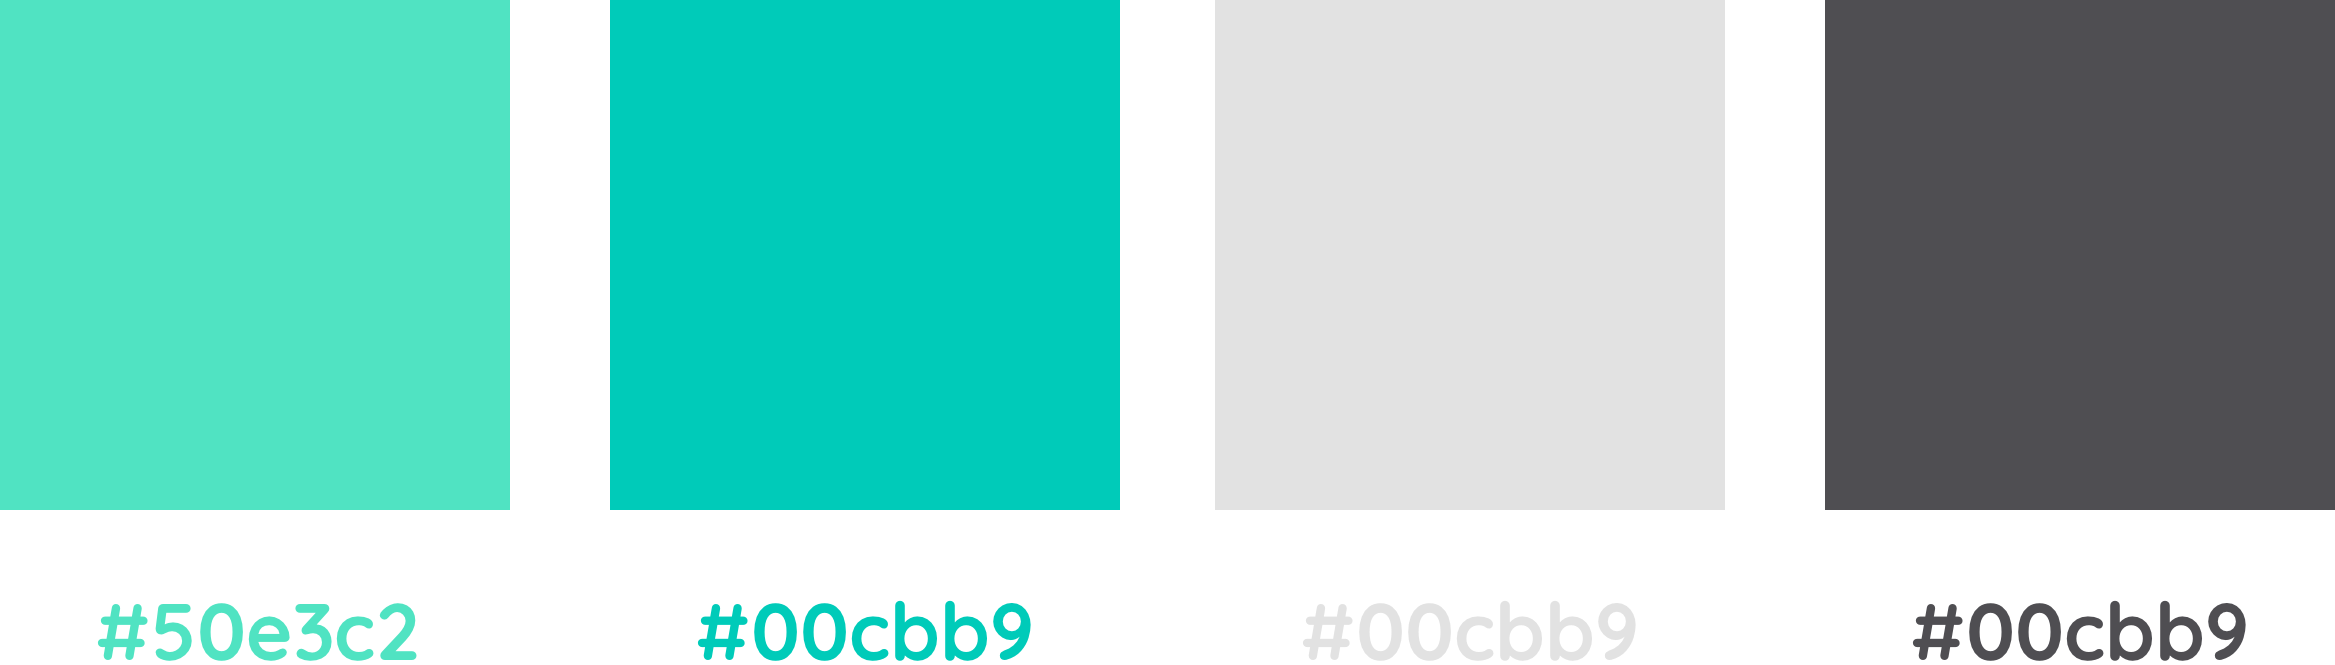
\includegraphics[width=0.68\textwidth]{img/colors.png}
\caption{Color palette.}
\label{colorpalette}
\end{figure}


\begin{figure}
\centering

\includegraphics[width=0.68\textwidth]{img/fonts.png}
\caption{Font Styles and .}
\label{fontstyles}
\end{figure}

%If a user wants to join an activity, it has to be easy to indicate their participation. 

\subsection{Features}

\subsection{Explorative Components}

\subsection{The Recommendation Algorithm}
\begin{itemize} 
	\item Wie sollen die Empfehlungen konkret gegeben werden? (Mit Codebeispielen)
	\item Andere Aktivitäten empfehlen, basierend auf bewertete Aktivitäten (explizit, kontextsensitiv)
\end{itemize} 
 % Autonomy of Decisions
% - *Allgemein:* Was soll der Ratgeber leisten? 
% - Sol sich nicht auf individuellen Rat verlassen.
% - Alle Beteiligten werden mit einbezogen.
% - Vorschläge geben und dem Nutzer die Entscheidung überlassen, ob er dieser nachgehen mag.
% - Besitzt nicht den Anspruch, dem Menschen die Entscheidungen abzunehmen. Auch deshalb, da die Aufgabe, Empfehlungen zu geben, nicht wohldefiniert ist, da diese zu vielschichtig ist.
% - Weiterhin bestehen geläufige Probleme der Empfehlungsalgorithmen, wie bspw. dem Cold Start und der Filterblase
	
\section{Required Hardware and Software}

\chapter{Empirical Method}

\section{Technical Validation}
\begin{itemize} 
	\item Beispielhaftes Modell und Anwendung des Algorithmus.
\end{itemize} 

\section{User-centered Validation}

\subsection{Recruitement}

\subsection{Participants}

\subsection{System Usability Score}
\begin{itemize} 
	\item Evaluation der Usability
	\item Ausschließen, dass Empfehlungen bewertet werden und nicht die Defizite der Applikation
\end{itemize} 

\subsection{Opening Questionnaire}

\subsection{Closing Questionnaire}
\begin{itemize} 
	\item Nutzerzentriertes Evaluieren der Empfehlungsalgorithmen.
	\item Ist es gelungen, die Freizeitgestaltung zu vereinfachen?
\end{itemize} 

\section{Structured Interview}
\begin{itemize} 
	\item Hast du mind. einen Streifzug unternommen?
	\item Hat es deine Freizeitgestaltung direkt oder indirekt beeinflusst (hatte es impact)?
\end{itemize}

\chapter{Results}

\section{Technical Validation}

\section{System Usability Score}

\section{Opening Questionnaire}

\section{Closing Questionnaire}

\section{Structured Interview}

\chapter{Analysis}
Ergebnisse der Studie wiederholen und in den Kontext stellen

\chapter{Conclusion}
\begin{itemize} 
	\item Thema, wie in der Einführung, aufgreifen
	\item Ausblick formulieren
	\begin{itemize} 
		\item Implementation von Bucketlisten?
	\end{itemize} 
\end{itemize} 


\appendix
\chapter{Appendix}
\newpage
\section{Studymaterial}
\vspace*{\fill}
%\center{\frame{\includegraphics[width=.98\textwidth, page=1]{apx/Studieninformationen}}}
\label{lab:Studymaterial}
\vspace*{\fill}

% Literaturverzeichnis
\clearpage
\pagenumbering{roman}
\bibliographystyle{mlu_ifg}
\bibliography{books}

%Abbildungsverzeichnis
\listoffigures

% Erklärung
\chapter*{Declaration of academic honesty}
\thispagestyle{empty}
XXXX
\begin{center}
\begin{tabular}{lp{2em}l} 
 \hspace{5cm}   && \hspace{4cm} \\\cline{1-1}\cline{3-3} 
 Bremen, \today    && Jan-Hendrik Wolf 
\end{tabular} 
\end{center}
\end{document}